% ============================================================================
% Experimental Setup
% ============================================================================

\subsection{Platform and Testbed}

\textbf{Rover.}
The mobile platform is a 13-DOF mobile manipulator: a 10-DOF rocker--bogie
base integrated with a 3-DOF robotic manipulator (Fig.~\ref{fig:rover}).
The rocker--bogie suspension maintains continuous wheel--ground contact on
uneven terrain without active suspension, making the system suitable for
sandy, planetary-analogue, and field environments.

\begin{figure}[t]
  \centering
  \IfFileExists{figures/rover.jpg}{%
    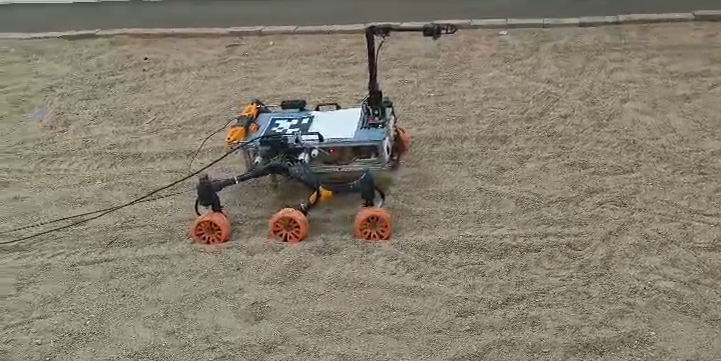
\includegraphics[width=0.85\columnwidth]{figures/rover.jpg}%
  }{%
    \fbox{\parbox{0.85\columnwidth}{\centering\vspace{2.0cm}
      \textit{[Rover photo --- save to paper/figures/rover.jpg]}
      \vspace{2.0cm}}}%
  }
  \caption{The 13-DOF mobile manipulator used in experiments:
  10-DOF rocker--bogie base with six passive wheels and a 3-DOF arm.
  Two UWB tags at \SI{50}{\centi\metre} baseline are mounted on the chassis;
  BNO085 IMU is co-located with Tag~1.}
  \label{fig:rover}
\end{figure}

\begin{figure}[t]
  \centering
  \IfFileExists{figures/setup_overview.jpg}{%
    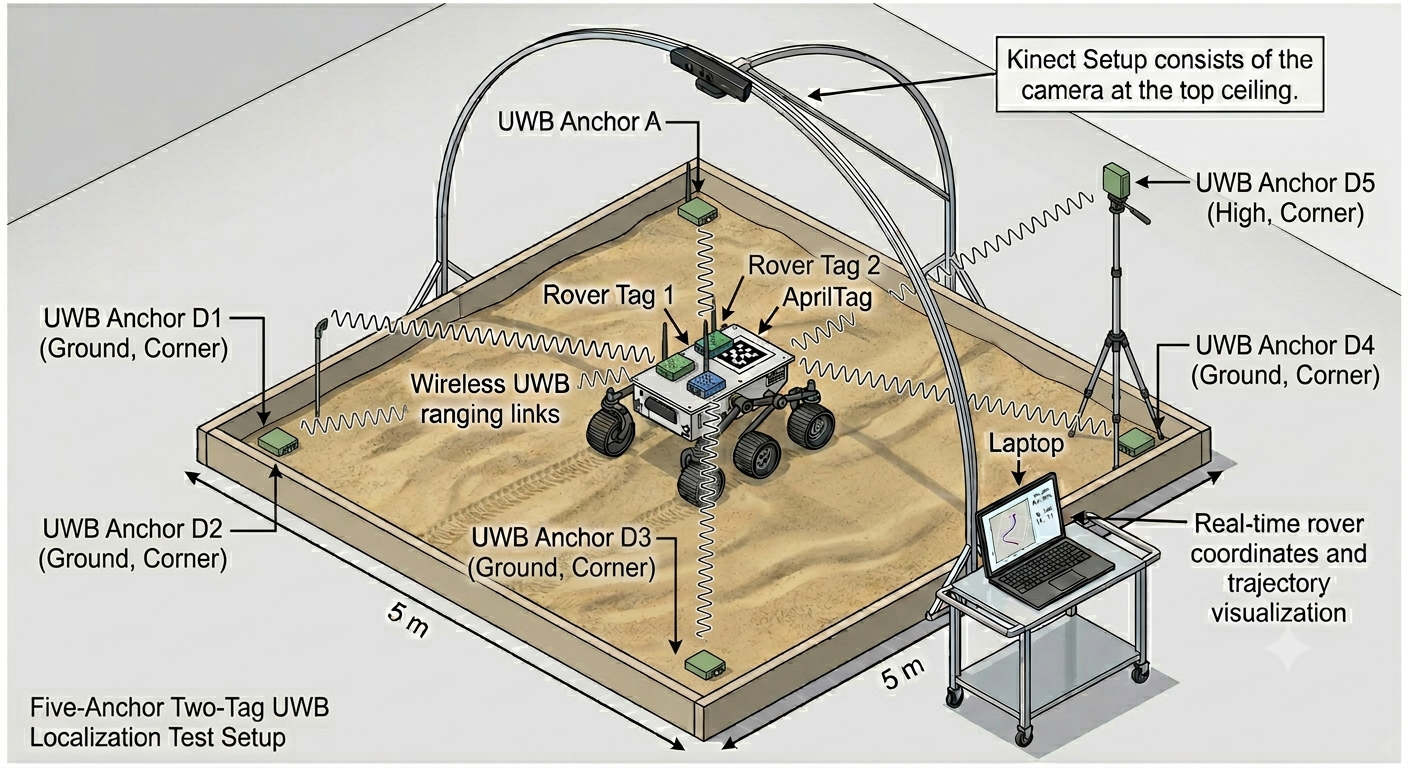
\includegraphics[width=\columnwidth]{figures/setup_overview.jpg}%
  }{%
    \fbox{\parbox{\columnwidth}{\centering\vspace{1.5cm}
      \textit{[Setup overview photo --- save to paper/figures/setup\_overview.jpg]}
      \vspace{1.5cm}}}%
  }
  \caption{Five-anchor two-tag experimental testbed in the
  $5\,\mathrm{m}\times5\,\mathrm{m}$ indoor sandbed.
  Anchors D1--D4 at ground corners, A elevated; rover carries Tags 1 and 2.
  Kinect~v2 (ceiling) provides ground-truth pose via AprilTag detection.}
  \label{fig:setup_overview}
\end{figure}

\textbf{Anchor deployment.}
Five anchors are deployed in a $5\,\text{m}\times5\,\text{m}$ sandbed
(Fig.~\ref{fig:topology}).
Anchors $A_1$--$A_4$ are coplanar near the floor;
$A_5$ is elevated at $h_e = 1.2$\,m.
Table~\ref{tab:anchor_positions} lists anchor coordinates.

\begin{table}[h]
  \centering
  \caption{Anchor positions (tape-measure ground truth).}
  \label{tab:anchor_positions}
  \begin{tabular}{lccc}
    \toprule
    Anchor & $x$ (m) & $y$ (m) & $z$ (m) \\
    \midrule
    $A_1$ (0x01) & 0.000 & 0.000 & \todo{} \\
    $A_2$ (0x02) & \todo{} & \todo{} & \todo{} \\
    $A_3$ (0x03) & \todo{} & \todo{} & \todo{} \\
    $A_4$ (0x04) & \todo{} & \todo{} & \todo{} \\
    $A_5$ (0x05) & \todo{} & \todo{} & 1.200 \\
    \bottomrule
  \end{tabular}
\end{table}

\subsection{Ground Truth System}

Ground truth is provided by a Microsoft Kinect~v2 depth camera
\cite{kinect_v2} mounted on the ceiling,
with an AprilTag marker board rigidly fixed to the rover.
The Kinect delivers RGB-D frames at \SI{30}{\hertz};
AprilTag pose estimation runs in real time using the \texttt{apriltag} library.
Ground-truth accuracy: \todo{X mm} in position, \todo{Y deg} in heading,
measured at known distances from the camera.

\textbf{Frame registration.}
The Kinect frame is aligned to the anchor world frame by a one-time
registration: the rover is placed at three known positions and the rigid
transform $\mathbf{T}_{\text{Kinect}\to\text{World}}$ is estimated from
corresponding 3D point pairs.
\todo{Report registration residual after alignment.}

\subsection{Experimental Protocol and Metrics}

\textbf{Scenarios.}
\textit{Static accuracy}: rover placed at $K = \todo{K}$ grid positions,
$M = \todo{M}$ sweeps collected at each.
\textit{Dynamic (primary)}: rover traverses \todo{describe path} at \todo{speed}\,m/s;
Kinect ground truth recorded at \SI{30}{\hertz} and resampled to sweep timestamps.
\textit{NLOS}: anchor \todo{A\_X} obstructed by \todo{obstacle type};
gap distributions and weighting effect recorded.
\textit{Sweep rate vs. anchor count}: $N \in \{3,4,5\}$ anchors measured
over 60\,s to verify linear scaling.

\textbf{Metrics.}
\begin{itemize}
  \item \textbf{2D/3D RMSE}: $\epsilon_{xy}$, $\epsilon_{xyz}$
  \item \textbf{Heading RMSE}: $\epsilon_\psi$ (dual-tag yaw vs.\ Kinect)
  \item \textbf{CDF of 2D error}: $P(\epsilon_{xy} < \epsilon)$;
    percentiles $\epsilon_{50}$, $\epsilon_{90}$, $\epsilon_{95}$
  \item \textbf{Sweep rate} and \textbf{end-to-end latency}
\end{itemize}
